\section{Materials and Methods}
\label{sec:methodology}

This review follows the PRISMA 2020 reporting guidelines~\cite{Page2021}, the
eight-step SLR process of Xiao and Watson~\cite{XiaoWatson2019}, a single-wave
adaptation of the citation-snowballing procedure of
Wohlin~\cite{Wohlin2014} (one forward/backward pass on the seed set, not iterated
to saturation; \S\ref{sec:conclusion:threats}), and general
SLR guidance from Kitchenham and Charters~\cite{KitchenhamCharters2007} and
Webster and Watson~\cite{Webster2002}. The review was
not prospectively registered in a review protocol repository. PROSPERO
restricts registration to reviews with a health-related outcome, which this
review does not have; general-purpose registries that do accept
computer-science and engineering review protocols (OSF Registries,
protocols.io) exist but were not used, the protocol evolved iteratively
rather than being fixed in advance, and every search string, screening rule,
and per-record decision is instead documented in Appendices~A--D and the
public pipeline repository (Data Availability). Retrospective registration was
considered and judged to add little beyond that documentation. The completed
PRISMA 2020 27-item checklist is provided as Supplementary Material. This
review was conducted and reported in accordance with the PRISMA 2020 statement.
The three intersecting fields covered are parameter-efficient fine-tuning (PEFT) and
adapter architectures; distributed and peer-to-peer (P2P) machine learning;
and multi-task LLM serving and inference. In accordance with the MDPI
Statement on the Use of Artificial Intelligence, the AI tools used and their
precise roles are disclosed here. Undermind (undermind.ai; accessed
2026-04-14) was used as a candidate-retrieval aid to assemble the six
thematically focused pre-validated groups (Appendix~\ref{app:undermind}); it
suggested candidate papers that the author then independently retrieved and
screened against the stated inclusion criteria. Two Anthropic Claude models
were used in strictly advisory roles inside the screening pipeline:
title-level triage of the 130-record single-keyword queue used Claude
Haiku~4.5 (model \texttt{claude-haiku-4-5-20251001}; term-set version~1.0),
which produced preliminary \textsc{include}/\textsc{exclude}/\textsc{uncertain}
suggestions that the author verified individually
(Appendix~\ref{sec:appendix:corpus_pipeline}, \S A.4), and abstract-level
review was accompanied by one-sentence advisory notes from Claude Sonnet
(\texttt{claude-sonnet-4-6}; \S A.7). Claude Sonnet models (Anthropic,
\texttt{claude-sonnet-4-6} through \texttt{claude-sonnet-5}), accessed
through the Claude Code interface between \textbf{2026-05-12} and
\textbf{2026-09-12}, were used as a drafting-assistance and copy-editing
aid under the author's direction. None of these tools made any
inclusion, exclusion, appraisal, or synthesis decision; the author conceived
the research questions, conducted the analysis and synthesis, made all
editorial decisions, verified all reported numbers against the underlying
pipeline data files, and assumes full responsibility for the content of this
article, including any errors or omissions. An earlier version of the search strategy
and screening protocol described in this section was developed as coursework
for a doctoral Research Methodology course at the University of Rijeka. That
version was submitted only for course assessment and was not deposited in an
institutional repository or otherwise published; the present manuscript has
been substantially revised and expanded from it.

\subsection{Search Strategy and Corpus}
\label{sec:methodology:search}

The search was anchored on nine foundational seed papers (Group G0,
Table~\ref{tab:g0_seeds}) selected
for direct cross-pillar relevance and demonstrated citation impact in
top-tier venues (e.g., LoRA and AdapterFusion each exceed 1,000 citations as
of August 2026; Petals, as a more recent 2023 system paper, has accumulated a
substantial and rapidly growing citation count). %CORRECTED 2026-08-30 (Blocking Issue #4, verified via
%mdpi_slr_engine/.../verify_prisma_counts.py cross-checked against the
%authoritative log_retrieval_2026-04-21.json, which records n_seeds=7 and
%lists exactly which seeds were submitted for backward/forward retrieval).
%An earlier pass at this fix wrongly inferred "not submitted" from the
%absence of a direction=SEED row for a seed in pipeline_unified.csv; that
%file's G0 bookkeeping is incomplete for Houlsby 2019 and Hu et al. 2022
%(LoRA), both of which log_retrieval_2026-04-21.json confirms WERE
%submitted (yielding 157 and 136 new records respectively) and both of
%which ARE rows in the final 123-record list, just not tagged as G0/SEED
%in pipeline_unified.csv's consolidation. The original manuscript text
%naming the two Sajina works as the ones NOT submitted was correct; the
%clarification below only adds their final-123 disposition, which the
%original text did not state.
Of these nine seeds, seven were submitted to the automated
citation-snowballing pipeline (Houlsby et al.\ 2019; Hu et al.\ 2022, LoRA;
Pfeiffer et al.\ 2020, AdapterHub; Pfeiffer et al.\ 2021, AdapterFusion;
Borzunov et al.\ 2023, Petals; Han et al.\ 2024; Sheng et al.\ 2024, S-LoRA);
the remaining two ({\v{S}}ajina et al.\ 2024; {\v{S}}ajina 2025) were not
submitted for automated retrieval and are cited as background and
motivating references only. \sloppy Of the seven submitted, six are themselves retained
as rows in the final 123-record corpus; the remaining one (Han et al.\ 2024) is
cited as a background and positioning reference only.
Table~\ref{tab:g0_disposition} records the
disposition of each seed. Six thematically focused
pre-validated groups (G1--G6) were assembled
by manual curation of leading venues (ACL, EMNLP, NeurIPS, ICML, MLSys);
Table~\ref{tab:groups} summarises their scope and contribution. Each group
was built from the exported relevance-ranked result list of one Undermind
deep search (queries run 2026-04-14, metadata corrected 2026-04-17;
reproduced verbatim in Appendix~\ref{app:undermind}): \textbf{377} records
across the six lists (G1~62, G2~42, G3~96, G4~56, G5~46, G6~75), reduced to
\textbf{343} after removing \textbf{34} records that also appeared in a
higher-priority group as cross-group duplicates, and joined by the nine G0
seeds to form the \textbf{352}-record pre-validated corpus. Every record on
these lists was assessed individually by the author against the eligibility
criteria of \S\ref{sec:methodology:eligibility} before entry; Undermind
supplied and ranked candidates but made no inclusion decision. Undermind
returns a relevance-ranked list rather than an exhaustive hit count, and the
size of the candidate pool it evaluated per query before producing each
exported list was not separately retained; this route is therefore reported
from its exported lists (377 records) rather than from a raw candidate pool,
a limitation on identification-stage audit granularity noted in
\S\ref{sec:conclusion:threats}. \textbf{105} of the final 123 records are
attributed to groups G1--G6 by the unified pipeline
(G1~17, G2~17, G3~14, G4~16, G5~11, G6~30), the remaining 18 to G0. This
count follows the pipeline's group label and is not a strict subset of the
343: the LoRA and Houlsby adapter papers entered as G0 seeds but were also
returned by the G1 and G2 searches and are booked under those groups here
(Table~\ref{tab:g0_disposition}). The per-group funnel is given in
Table~\ref{tab:groups} and Appendix~\ref{sec:appendix:corpus_pipeline}, \S A.1.
Forward and
backward citation snowballing on G0 was executed via the Semantic Scholar API
on 2026-04-21, supplemented by a Scopus/WoS forward pass on 2026-05-08.
\fussy After deduplication, \textbf{972 unique records} entered title screening, of
which \textbf{162} passed; these screened-in records were merged with the
352-paper pre-validated corpus (G0--G6): 162 + 352 = 514 candidate records, of
which 12 were removed as duplicates already present in both the newly-screened
set and the pre-validated corpus, yielding the reported \textbf{502}-record
corpus. A dedicated search for competing secondary studies (systematic
reviews, surveys, and taxonomies) of overlapping scope was run in addition to
the primary retrieval; its method and result are given in the \emph{Related
reviews and surveys} paragraph below and Table~\ref{tab:related_surveys}.
Surveys and reviews that also surfaced during the primary retrieval and
snowballing were screened under the same eligibility criteria and retained as
corpus records where they qualified (study-type breakdown in
\S\ref{sec:methodology:eligibility}). Enrichment and a topical-relevance/tier filter
retained \textbf{464} records. Abstract review across two passes covered these
464 records plus \textbf{88} records added by a supplementary forward-citation
snowball pass (Scopus and WoS), yielding a combined abstract-review pool of
\textbf{552}; of these, \textbf{214} were classified KEEP and exported for
full-text review, \textbf{173} were classified DEFER and carried into the
full-text queue for closer inspection, and the remaining \textbf{165} were
classified SKIP and did not proceed further. The \textbf{88} supplementary forward-snowball records
resolved at this second abstract-review pass as \textbf{12} KEEP, \textbf{4}
DEFER, and \textbf{72} SKIP. The 12 KEEP records entered the full-text queue
(8 reaching data extraction), yet none of the 88 \texttt{G\_SNOW\_F} records
survived to the final list; the supplementary forward branch therefore
contributed \textbf{0} of the 123 final records. Summed across identification
routes --- the 1,150-record snowball retrieval, the 377-record Undermind
G1--G6 exports, the 9 direct G0 seeds, the 88-record supplementary
forward-citation snowball, and the 34-record manual cross-validation top-up
--- \textbf{1,658} gross records were identified before any cross-route
deduplication. %CORRECTED 2026-08-30 (Blocking Issue #2, verified via
%mdpi_slr_engine/.../verify_prisma_counts.py): the abstract-review pipeline records
%only a coarse KEEP/SKIP disposition and does not retain an individually
%coded exclusion reason for SKIP records; these 165 exclusions are disclosed
%here as a named limitation (\S\ref{sec:conclusion:threats}) rather than
%itemised by cause, consistent with PRISMA 2020 Item 16b.
The abstract-review pipeline records only a coarse KEEP/SKIP disposition and
does not retain an individually coded exclusion reason for SKIP records; this
gap is disclosed as a named limitation in
Section~\ref{sec:conclusion:threats} rather than papered over. The full-text
review queue therefore comprises \textbf{387} records (214 KEEP
${}+{}$ 173 DEFER). Of these, \textbf{190} (all KEEP-origin; no DEFER-origin
records reached extraction) underwent data extraction; the remaining
\textbf{197} (24 KEEP-origin, full text unavailable; 173 DEFER-origin, not
taken further) were excluded.
%CORRECTED 2026-08-30 (Blocking Issue #3): the extraction-stage total of 224
%is not a linear 387-minus-exclusions subtraction; a supplementary manual
%Scopus/WoS cross-validation search contributed 34 further records extracted
%in parallel, entering directly at the extraction stage without ever passing
%through the 387-record full-text queue (verified: all 34 have no S5/S6/S7b/Q9
%stage flags set in pipeline_unified.csv). None of the 34 were ultimately
%retained in the final 123-record list.
A supplementary manual Scopus/WoS cross-validation search contributed
\textbf{34} further records extracted in parallel, entering directly at the
extraction stage without passing through the full-text queue; none of these
34 were ultimately retained in the final 123-record list. The extraction-stage
total is therefore \textbf{224} (190 ${}+{}$ 34). Full-text reading and quality assessment
then reduced the corpus to \textbf{123 papers} (2002--2026); these correspond
to \textbf{120 distinct papers}\footnote{The count of 123 includes 120 distinct
papers because three works are each recorded as two separate entries in the
data files. Two foundational works are each recorded under both their arXiv
and Scopus retrieval keys: LoRA (arXiv 2106.09685 and Scopus a8ca46\ldots) and
the original adapter-based parameter-efficient transfer-learning method (arXiv
1902.00751 and Scopus 29ddc1\ldots). A third work, CaraServe~\cite{Li2024CaraServe},
was retrieved twice under different identities: once as its 2024 arXiv
preprint, and again as its 2025 peer-reviewed publication at USENIX ATC, where
it was renamed ``Toppings.'' The final reading list therefore contains
123 rows corresponding to 120 unique studies.}, because two foundational works
(LoRA and the original adapter-based parameter-efficient transfer-learning
method) are each recorded under both their arXiv and Scopus retrieval keys in
the reading list, and a third work (CaraServe, later published as Toppings)
was retrieved separately as its preprint and its renamed publication.
The 123 final records break down by \emph{discovery route} --- targeted
pre-validated retrieval, citation snowballing, and direct seeds --- in
Table~\ref{tab:discovery_route}. The \textbf{101} records that entered the
extraction stage (\textbf{224}) but were not retained in the final reading list
(\textbf{123}) divide into three eligibility-stage categories that sum to 101:
\textbf{34} manual Scopus/WoS cross-validation top-up records (which, as noted
above, contributed no final records), \textbf{53} background-corpus records
retained for context but excluded before the final list, and \textbf{14}
core-corpus records that did not pass full-text inclusion appraisal
(Table~\ref{tab:final_exclusions}). This funnel is summarised in
Figure~\ref{fig:prisma} and traceable record-by-record through the unified
pipeline file (Appendix~\ref{sec:appendix:corpus_pipeline}).

\paragraph{Related reviews and surveys.}
A dedicated search for competing secondary studies was run on \textbf{2026-09-10}
across Web of Science (Core Collection, topic field \texttt{TS=}) and Scopus
(\texttt{TITLE-ABS-KEY}, document type \texttt{re}), restricted to 2021--2026;
the two query strings are reproduced in Appendix~\ref{app:db_queries}. The
searches returned \textbf{50} (WoS) and \textbf{19} (Scopus) records. After
removing false positives (predominantly the LoRa long-range radio protocol,
hardware ``adapters'', and application-domain reviews in medicine and IoT)
and applying the inclusion rule (a secondary study whose stated scope covers at
least two of this review's five pillars), \textbf{six} distinct competing
surveys were retained \emph{for positioning}; one further survey known to the
author but indexed in neither database, Pfeiffer et
al.~\cite{PfeifferModular2023}, was added on the same criterion. These seven
surveys are used only for the comparison in Table~\ref{tab:related_surveys} and
are \emph{not} part of the 123-record evidence corpus, which is built solely
from the primary retrieval and snowballing described above.
Table~\ref{tab:related_surveys} maps their pillar coverage.
None of the seven covers the five pillars jointly, and none takes
decentralised, coordinator-free adapter exchange as its subject: the federated
surveys~\cite{WoisetschlagerFLsurvey2024,YangFedLoRAsurvey2025} treat adapter
\emph{co-training} under a coordinating server; the edge and general-LLM
surveys~\cite{JiangEdgeLLM2026,LukacLLMsurvey2026} treat adapters as a
personalisation technique within single-operator or edge--cloud deployments;
the agentic-edge survey~\cite{DibAgenticEdge2026} includes a peer-to-peer
topology but at the level of agent messages and gradients, not adapters; and
the modular-learning survey~\cite{PfeifferModular2023} covers adapter
composition and routing thoroughly but centrally. The synthesis in this review
occupies the unfilled cell of Table~\ref{tab:related_surveys} (placed with the
other corpus tables below).

\paragraph{Disconfirming (adversarial) search.}
Because the review's central contribution is a gap claim, a structured search
for disconfirming evidence was run on \textbf{2026-09-10} following the
grey-literature review guidelines of Garousi et al.~\cite{Garousi2019}: eight
queries across arXiv, GitHub, and general web search, with no peer-review or
venue filter, seeking any system, protocol, or project that treats adapters as
the unit of exchange over a frozen shared backbone under a coordinator-free
peer-to-peer topology (queries, sources, screening rule, and results in
Appendix~\ref{app:db_queries}, \S~C.4). No located artefact provides that
combination together with decentralised capability discovery and multi-adapter
composition; the nearest candidates each address a single facet:
decentralised serving of \emph{whole} models (e.g.\ PlanetServe, Platformless
AI), decentralised co-training of a \emph{single} shared adapter
(Dec-LoRA~\cite{Ghiasvand2025} and related work), centralised adapter
retrieval-and-composition (the LoraRetriever~\cite{ZhaoLoraRetriever2024}
line), and DHT capability discovery for \emph{agents} rather than adapters. This
supersedes the informal counter-search reported in
\S\ref{sec:conclusion:threats} and places the \S\ref{sec:synthesis_gap} gap
claim on a documented basis.

\paragraph{Post-review top-up search.}
In response to peer review, a supplementary search was run on
\textbf{2026-09-12} to check for relevant literature published after the
original search's cutoff, covering Scopus, Web of Science, and arXiv with
the same Boolean queries used throughout (year bound moved forward to the
gap window; queries, screening, and results in
Appendix~\ref{app:db_queries}, \S~C.5, and Appendix~\ref{app:search_log},
\S~D.7). The three sources returned 93 distinct candidates after
deduplication; a title/abstract screen at the same depth as this review's
own Layer-2 stage retained 65; author eligibility review against the
criteria of Table~\ref{tab:inclusion_exclusion} (applying I4 strictly ---
peer-reviewed venue required, since no citation-count check was performed on
the arXiv-only survivors) retained \textbf{four}: DyMerge-LoRA
\cite{XuDyMergeLoRA2026}, AdaFuse~\cite{LiAdaFuse2026},
TailorLLM~\cite{WangTailorLLM2026}, and DeCAF~\cite{SaadatiDeCAF2026}, cited
where relevant in Sections~\ref{sec:inference_systems},
\ref{sec:moe_routing}, and \ref{sec:p2p_federated}. These four are discussed
narratively only: unlike the primary corpus, they were not put through
Wohlin snowballing, quality appraisal, or discovery-route classification,
and are excluded from the 123-record corpus and every statistic derived
from it (Table~\ref{tab:discovery_route}, Table~\ref{tab:quality_rubric}, the
concept matrix of \S\ref{sec:synthesis_gap}, and the Boolean-recall check of
\S\ref{sec:appendix:corpus_pipeline}). The PRISMA flow diagram
(Figure~\ref{fig:prisma}) reports the original search only, consistent with
its function as an audited record of that process; this top-up search is
reported here and in Appendices C.5/D.7 instead of being retrofitted into it.

\paragraph{Scope of the coded extraction.}
The archived data-extraction table (224 rows,
Appendix~\ref{sec:appendix:corpus_pipeline}, Table~\ref{tab:extraction_codebook})
records bibliographic and classificatory fields: record key, DOI, title,
authors, year, venue, citation count, reading-priority tier, review source,
corpus position, contribution type, PEFT technique, distribution mechanism,
citing review sections, and contribution codes, together with free-text
\texttt{key\_finding} and \texttt{notes\_raw} columns holding full-text reading
notes. The three columns intended to hold structured evaluation data
(\texttt{method\_name}, \texttt{datasets}, \texttt{metrics}) are uniformly empty
in the archived export. The comparative synthesis in
Sections~\ref{sec:peft}--\ref{sec:synthesis_gap} was therefore produced by
narrative full-text reading and is documented in the free-text notes and in
Table~\ref{tab:datasets} (33 systems checked directly against their primaries),
not derived from coded quantitative fields.

\subsection{Eligibility Criteria}
\label{sec:methodology:eligibility}

Records were eligible for inclusion if they addressed at least one of the
three review themes (PEFT/adapters, distributed or P2P/federated machine
learning, or multi-task LLM serving/inference). Two pre-2021 restrictions
that apply to snowballed records do \emph{not} apply to the pre-validated
G0--G6 corpus, which was assembled by manual curation and deliberately
bypasses the year filter to capture pre-PEFT-era foundational works
(e.g.\ Houlsby et al.\ 2019, Hu et al.\ 2022). Specifically:
(i) only English-language records were retained;
(ii) snowballed records were required to have a publication year
$\geq$2021, chosen because the confluence of LoRA and large-scale transformer
deployment marks the practical onset of the PEFT-at-scale era addressed by
this review;
(iii) peer-reviewed conference and journal papers were preferred, and
arXiv preprints were retained only where they carried a non-trivial external
citation count (Semantic Scholar, retrieved at search time) as a minimal,
external proxy for community engagement and peer scrutiny
(Appendix~\ref{sec:appendix:corpus_pipeline}, \S A.3--A.4). The full criteria
and their motivations are detailed in the appendix. With respect to study type,
the 120 distinct papers underlying the 123 included records (three works:
LoRA, Houlsby et al., and the CaraServe/Toppings pair, each appear as two
records; \S~\ref{sec:methodology:search}) comprise \textbf{111} primary studies
(PEFT methods, serving systems, composition mechanisms, and federated/P2P
training schemes) and \textbf{9} survey or overview contributions ($7.5\%$)
retained to establish field context and to map the taxonomy, and no position or
tutorial works are included among the 120. Counted at the level of the 123
records rather than the 120 distinct papers, the split is 114 primary / 9
survey.

\subsection*{Screening Reviewer Configuration}
\label{sec:methodology:screening_reviewers}

Title, abstract, and full-text screening in this review were conducted by
a single reviewer (the author), consistent with the disclosure requirement
of PRISMA 2020 Item~8~\cite{Page2021}, which requires reporting the number
of reviewers involved in the selection process but does not mandate dual
independent screening as a condition of compliance. Dual independent
screening is widely recommended as best practice in systematic review
methodology~\cite{KitchenhamCharters2007} and is treated as mandatory in
some domain-specific frameworks for full-text inclusion decisions (e.g.,
Cochrane/MECIR standard C39); however, single-reviewer execution remains
an accepted and common practice for single-author systematic reviews in
computer science, particularly doctoral-level work conducted without a
research team~\cite{KitchenhamCharters2007}. No second independent human
reviewer was available for this review, and none was recruited for
screening. Consequently, no inter-rater reliability statistic (e.g.,
Cohen's $\kappa$) is reported for the screening process: a reliability
coefficient computed against a non-independent artefact (such as an
automated classifier sharing the same review pipeline and inclusion
rubric as the primary screener) would not constitute a valid measure of
independent human agreement, and reporting one risks implying a
validation that was not in fact performed.

% --- Internal-validity note (single-reviewer screening) -----------------------
% Resolved 2026-09-10: disclosure-only. This is a single-author doctoral SLR;
% no independent second human screener was available. PRISMA 2020 Item 8 asks
% for the reviewer count, not dual screening, and a kappa computed against the
% non-independent automated classifier would not be a valid agreement measure
% (both points are made in the prose above and in the Threats to Validity
% section). A 5-10 percent blind re-screen -- by a colleague, or a delayed
% self re-screen for intra-rater agreement -- was considered and not undertaken
% before submission; the limitation is disclosed as reported rather than
% measured. Kept as source comment for the record; not rendered.
% ---------------------------------------------------------------------------

This single-reviewer limitation applies specifically to the screening and
appraisal of the snowball-retrieved candidate pool. The six thematically
pre-validated groups (G1--G6, Appendix~\ref{app:undermind}), which
contribute 105 of the 123 final records (85.4\%), were assembled via targeted,
framing-informed retrieval rather than blind snowball screening; this
route avoids the screening-reliability risk discussed above, but
introduces a distinct risk of confirmation bias in candidate discovery,
since retrieval queries were constructed with prior knowledge of the
review's own pillar structure and target systems. Both risks are
therefore acknowledged as complementary, not mutually mitigating: the
curated-corpus route reduces exposure to inconsistent single-reviewer
screening but does not reduce, and may compound, the risk of a
retrieval process shaped by the review's own hypotheses. This is
discussed further in Section~\ref{sec:conclusion:threats}.

A group label (G0--G6) records the corpus into which a paper was finally
placed, not how it was discovered; G0's final count in particular folds in
14 citation-snowball descendants (Table~\ref{tab:groups}). The split by
\emph{discovery route}, taken from the unified pipeline's \texttt{direction}
field, is reported separately in Table~\ref{tab:discovery_route}. Two G0 seed
papers -- Houlsby et al.~\cite{Houlsby2019} and Hu et al.~\cite{Hu2022}
(LoRA) -- are attributed by group label to G2 and G1 respectively rather than
to G0, and each is present in the pipeline as two rows (an arXiv-sourced and
a Scopus-sourced record); their group-label total and their discovery-route
\texttt{direction=PREVALIDATED} tally therefore share the same four
seed-origin rows, so agreement between the two counts does not by itself
establish that the targeted-retrieval figure is free of seed influence.
Counting seed origin consistently gives \textbf{101} genuinely independent
targeted-retrieval records, \textbf{8} seed-origin rows (the four
directly-seeded records plus these four Houlsby/LoRA rows), and \textbf{14}
citation-snowball records, summing to 123 (Table~\ref{tab:discovery_route});
the two supplementary manual passes (the 88-record Scopus/WoS forward-snowball
pass and the 34-record cross-validation top-up) retained none.

Of the 123 included records, \textbf{70} (56.9\%) carry the extraction-document
\texttt{review\_source} label \texttt{fulltext}, and the remaining \textbf{53}
(43.1\%) carry the label \texttt{abstract-2nd-pass}. Both labels describe
records that passed through the same pipeline stages: all 123, without
exception, are members of the \textbf{387}-record full-text queue and its
\textbf{190}-record extraction subset in Figure~\ref{fig:prisma}
(\texttt{in\_fulltext\_queue\_Q9} = 1 and \texttt{in\_extraction\_E11} = 1 for
all 123 in the unified pipeline; verified in
\texttt{verify/wp13\_inclusion\_route\_membership.py}). \texttt{review\_source}
records which internal screening pass produced the eligibility decision --
an initial full-text read (\texttt{fulltext}) or a second abstract-level
pass that preceded it (\texttt{abstract-2nd-pass}) -- not a difference in
which pipeline stages the record reached. The 53 \texttt{abstract-2nd-pass}
records are drawn from the pre-validated/enriched corpus (G0--G6); none of
the 123 final records originates from the supplementary forward-citation
snowball pass, which contributed 0 records to the final list
(\S\ref{sec:methodology:search}). The
123 records (120 distinct papers) are distributed across the three
reading-priority tiers as \textbf{48} Tier-1, \textbf{42} Tier-2, and
\textbf{33} Tier-3 records (Figure~\ref{fig:tiers}, Appendix A). This
final-stage tiering re-classifies records at the level of the 123-record
reading list and is distinct from the earlier tier classification applied to
the 464-record enriched pool (90 Tier-1 / 141 Tier-2 / 233 Tier-3,
Table~\ref{tab:tiers}) at the enrichment stage;
papers may be re-tiered between stages as additional full-text and extraction
information becomes available.

\begin{table}[H]
\centering
\caption{The nine foundational seed papers (Group G0) and their role in the
review. Venues as recorded in the pre-validated corpus.}
\label{tab:g0_seeds}
\small
\setlength{\tabcolsep}{4pt}
\begin{tabular}{
  >{\raggedright\arraybackslash}p{0.20\textwidth}
  >{\raggedright\arraybackslash}p{0.24\textwidth}
  >{\raggedright\arraybackslash}p{0.44\textwidth}}
\toprule
\textbf{Seed} & \textbf{Venue} & \textbf{Role in this review} \\
\midrule
Houlsby et al.\ 2019 & ICML 2019 & Defines the bottleneck-adapter
paradigm; architectural baseline for modular adapters. \\
Hu et al.\ 2022 (LoRA) & ICLR 2022 & Primary PEFT method; P2P nodes
exchange low-rank matrices over a shared backbone. \\
Pfeiffer et al.\ 2020 (AdapterHub) & EMNLP 2020 & Centralised adapter
registry---the centralised analog of the peer-to-peer marketplace. \\
Pfeiffer et al.\ 2021 (AdapterFusion) & EACL 2021 & Composition mechanism
for mixture-of-adapter systems. \\
{\v{S}}ajina et al.\ 2024 & Future Gener.\ Comput.\ Syst.\ (Q1) &
Multi-task P2P learning on a shared transformer encoder; closest published
predecessor. \\
{\v{S}}ajina 2025 & Doctoral thesis, Univ.\ of Rijeka & Theoretical
foundation of P2P collaborative training without a central server. \\
Borzunov et al.\ 2023 (Petals) & ACL 2023 (Syst.~Demos.) & Only peer-reviewed,
deployed P2P frozen-backbone LLM inference system. \\
Han et al.\ 2024 & TMLR 2024 & PEFT survey; primary positioning reference. \\
Sheng et al.\ 2024 (S-LoRA) & MLSys 2024 & State-of-the-art multi-tenant
LoRA-serving baseline. \\
\bottomrule
\end{tabular}
\end{table}

%ADDED 2026-08-30 (Blocking Issue #4, verified via
%mdpi_slr_engine/.../verify_prisma_counts.py against log_retrieval_2026-04-21.json
%(the authoritative n_seeds=7 record of which seeds were submitted for
%automated backward/forward retrieval) and 13_final_reading_list_2026-05-12.csv:
%explicit per-seed disposition table, since Table~\ref{tab:g0_seeds} alone
%does not disclose which of the nine seeds are themselves rows in the final
%123-record corpus.
\begin{table}[H]
\centering
\caption{Disposition of the nine G0 seeds: whether each was submitted for
automated backward/forward retrieval, and whether it is itself a row in the
final 123-record corpus. The ``new records found'' figures are incremental
post-deduplication counts; their sum (972) matches the screened record total in
Table~\ref{tab:screening}. Verified against \texttt{\seqsplit{log\_retrieval\_2026-04-21.json}}
and the final reading list.}
\label{tab:g0_disposition}
\small
\setlength{\tabcolsep}{4pt}
\begin{tabular}{
  >{\raggedright\arraybackslash}p{0.24\textwidth}
  >{\raggedright\arraybackslash}p{0.10\textwidth}
  >{\raggedright\arraybackslash}p{0.54\textwidth}}
\toprule
\textbf{Seed} & \textbf{In 123?} & \textbf{Route / detail} \\
\midrule
Houlsby et al.\ 2019 & Yes & Automated retrieval (157 new records found); 2 rows in the final list (arXiv 1902.00751 and a distinct Scopus key), tier 2. \\
Hu et al.\ 2022 (LoRA) & Yes & Automated retrieval (136 new records found); 2 rows in the final list (arXiv 2106.09685 and a distinct Scopus key), tier 2. \\
Pfeiffer et al.\ 2020 (AdapterHub) & Yes & Automated retrieval (128 new records found); 1 row (arXiv 2007.07779), tier 2. \\
Pfeiffer et al.\ 2021 (AdapterFusion) & Yes & Automated retrieval (125 new records found); 1 row (2005.00247). \\
{\v{S}}ajina et al.\ 2024 (FGCS) & No & Not submitted for automated retrieval; cited as the closest published predecessor (background/motivation only). \\
{\v{S}}ajina 2025 (doctoral thesis) & No & Not indexed in the bibliographic databases used for automated retrieval; cited as theoretical background only. \\
Borzunov et al.\ 2023 (Petals) & Yes & Automated retrieval (131 new records found); 1 row (arXiv 2209.01188). \\
Han et al.\ 2024 (survey) & No & Automated retrieval (163 new records found), but the seed paper itself was not retained; cited as a positioning/background reference only. \\
Sheng et al.\ 2024 (S-LoRA) & Yes & Automated retrieval (132 new records found); 1 row (arXiv 2311.03285). \\
\bottomrule
\end{tabular}
\end{table}

A threat to construct validity deserves explicit acknowledgment: the nine G0
seeds were deliberately chosen at the \emph{intersection} of the three pillars
studied (PEFT, P2P collaboration, and multi-task serving), on the rationale of
cross-pillar relevance and high citation impact, assessed qualitatively
rather than against a fixed numerical threshold, in top-tier venues. Because this selection was informed by the research
question itself, it carries an inherent risk of biasing the corpus toward the
review's intended narrative and could under-sample works that challenge the premise of
decentralised adapter sharing. Two features mitigate this risk. First, the G0
set is complemented by the independently curated G1--G6 groups, which were
assembled from leading venues without reference to the seeds'
conclusions~\cite{XiaoWatson2019} (Table~\ref{tab:groups}). Second, forward and
backward citation snowballing and the Scopus/WoS forward pass expand the corpus
beyond the seeds' immediate frame. The nine G0 seeds were selected
qualitatively for citation impact rather than against a single fixed
numerical threshold applied uniformly at selection time; no such fixed
threshold was retained as an auditable selection parameter. To ground this
qualitative characterization, current citation counts were checked
informally at the time of writing (August 2026): the most established seeds
(LoRA, AdapterFusion) each exceed 1,000 citations, while more recent seeds
(e.g., Petals, published 2023) show lower but still substantial and rapidly
growing citation counts consistent with their shorter time in circulation.
These figures reflect the state of citation databases at the time of
writing rather than the original decision-time assessment, and are reported
to characterize impact qualitatively rather than to claim a precisely
audited, uniformly-applied threshold.

\begin{table}[H]
\centering
\caption{Pre-validated corpus groups: identification funnel, scope, and review section coverage. \emph{U.\ export} is the number of records in the exported relevance-ranked result list of each group's Undermind deep search (queries run 2026-04-14; Appendix~\ref{app:undermind}); 34 records that also appeared in a higher-priority group were removed as cross-group duplicates, reducing the 377 G1--G6 exports to 343, which with the 9 G0 seeds gives the 352-record pre-validated corpus. \emph{n}~pre-val.\ is the per-group count after that dedup. Undermind evaluates a larger candidate pool per query than it returns in the exported list; that pre-export pool size was not separately retained (\S\ref{sec:conclusion:threats}). Each final record is attributed to the single pre-validated group recorded by the unified pipeline; the \emph{n}~final column therefore partitions the 123-record total. G0's \emph{n}~final = 18 comprises four directly-seeded records (S-LoRA, AdapterHub, AdapterFusion, Petals) and 14 snowball descendants; two further seeds (Houlsby~2019, Hu/LoRA~2022) are in the final list but attributed outside G0 (Table~\ref{tab:g0_disposition}; see note below the table).}
\label{tab:groups}
\begin{tabular}{lp{4.4cm}rrrl}
\toprule
\textbf{Group} & \textbf{Theme} & \textbf{U.\ export} & \textbf{\textit{n} pre-val.} &
\textbf{\textit{n} final} & \textbf{Section(s)} \\
\midrule
G0 & Foundational seeds (PEFT, P2P, serving) & ---  & 9   & 18  &
\ref{sec:peft}--\ref{sec:adapter_composition}, \ref{sec:inference_systems} \\
G1 & PEFT methods beyond adapters and LoRA   & 62  & 59  & 17  & \ref{sec:peft} \\
G2 & Adapter composition for multi-task NLP  & 42  & 37  & 17  &
\ref{sec:adapter_composition} \\
G3 & Decentralised and P2P ML systems        & 96  & 95  & 14  &
\ref{sec:p2p_federated} \\
G4 & Adapter multiplexing for LLM inference  & 56  & 51  & 16  &
\ref{sec:inference_systems} \\
G5 & Routing and MoE for modular PEFT        & 46  & 35  & 11  &
\ref{sec:moe_routing} \\
G6 & Federated PEFT for transformer NLP      & 75  & 66  & 30  &
\ref{sec:p2p_federated} \\
\midrule
\textbf{Total} & & \textbf{377} & \textbf{352} & \textbf{123} & \\
\bottomrule
\multicolumn{6}{p{0.95\linewidth}}{\footnotesize The G0 \emph{n}~final of 18
is not 18 of the original nine seeds: it is the number of final-list records
attributed to group G0 by the unified pipeline, comprising 4 records whose
primary route is the seed itself (S-LoRA, AdapterHub, AdapterFusion, Petals)
plus 14 snowball descendants (10 forward, 4 backward). Two further G0 seeds
Houlsby et al.\ 2019 and Hu et al.\ 2022 (LoRA), are themselves in the
final list, but the unified pipeline attributes their records to G1 (LoRA) and
G2 (Houlsby), both papers were also returned by those groups' Undermind
searches rather than to G0, so their seed status is recorded only in
Table~\ref{tab:g0_disposition}. The nine seeds are listed in
Table~\ref{tab:g0_seeds}.} \\
\end{tabular}
\end{table}

\begin{table}[H]
\centering
\caption{This review against the closest competing secondary studies, by pillar
coverage. Consolidates every prior review or survey-like study named anywhere
in this manuscript: both the works cited in Section~\ref{sec:introduction} as
motivating the gap and those identified by the dedicated related-reviews
search (2026-09-10; \S\ref{sec:methodology:search}; query strings in
Appendix~\ref{app:db_queries}).
Columns: \emph{PEFT} = PEFT/adapters; \emph{Comp.} = adapter composition;
\emph{Serve} = multi-tenant serving; \emph{MoE} = MoE/routing;
\emph{P2P} = P2P/federated; \emph{Exch.} = decentralised, coordinator-free
adapter exchange (discovery, retrieval, composition) as the study's subject.
\checkmark~= substantive treatment; $\circ$~= partial or incidental; blank~= not
covered.}
\label{tab:related_surveys}
\small
\setlength{\tabcolsep}{4pt}
\begin{tabular}{l p{2.3cm} *{6}{c}}
\toprule
\textbf{Secondary study} & \textbf{Focus} & \textbf{PEFT} & \textbf{Comp.} &
\textbf{Serve} & \textbf{MoE} & \textbf{P2P} & \textbf{Exch.} \\
\midrule
Han et al.\ 2024~\cite{Han2024} & PEFT, comprehensive survey &
\checkmark & & $\circ$ & & & \\
Wang et al.\ 2024~\cite{WangAIReview2024} & PEFT, survey of methodologies &
\checkmark & & & & & \\
Mao et al.\ 2024~\cite{MaoLoraSurvey2024} & LoRA survey &
\checkmark & \checkmark & $\circ$ & & \checkmark & \\
{\v S}ajina et al.\ 2024~\cite{SajinaP2PConnection2024}\textsuperscript{a} &
autonomous P2P connection establishment & & & & & \checkmark & \\
Pfeiffer et al.\ 2023~\cite{PfeifferModular2023} & modular deep learning &
\checkmark & \checkmark & & \checkmark & & \\
Woisetschl{\"a}ger et al.\ 2024~\cite{WoisetschlagerFLsurvey2024} &
efficient FL for FMs & \checkmark & & & & \checkmark & \\
Yang et al.\ 2025~\cite{YangFedLoRAsurvey2025} & federated LoRA (FedLoRA) &
\checkmark & & & & \checkmark & $\circ$ \\
Dib 2026~\cite{DibAgenticEdge2026} & agentic edge intelligence &
$\circ$ & & $\circ$ & & \checkmark & \\
Jiang et al.\ 2026~\cite{JiangEdgeLLM2026} & edge LLMs &
\checkmark & & \checkmark & & $\circ$ & \\
Luk{\'a}{\v c} et al.\ 2026~\cite{LukacLLMsurvey2026} &
unified LLM survey & \checkmark & & & \checkmark & $\circ$ & \\
\midrule
\textbf{This review} & decentralised adapter-based inference &
\checkmark & \checkmark & \checkmark & \checkmark & \checkmark & \checkmark \\
\bottomrule
\multicolumn{8}{@{}p{\textwidth}@{}}{\footnotesize\textsuperscript{a}~Framed
as an overview but structured as an empirical comparison of specific
connection-establishment methods rather than a literature survey; included
here for pillar-coverage completeness since it is cited in
Section~\ref{sec:introduction} as part of the prior-work landscape.} \\
\end{tabular}
\end{table}

\begin{table}[H]
\centering
\caption{The 123 final records by \emph{discovery route}, from the unified
pipeline's \texttt{direction} field and independent of the group label in
Table~\ref{tab:groups}. ``Targeted retrieval'' is the Undermind-assisted
curation of Groups G1--G6, excluding four rows attributable to G0 seed papers
(see below); ``seed-origin'' is the four seeds submitted for retrieval in
their own right (S-LoRA, AdapterHub, AdapterFusion, Petals) plus two further
G0 seeds, Houlsby et al.\ and LoRA, each present as two rows (an
arXiv-sourced and a Scopus-sourced record) attributed by group label to G2
and G1 respectively rather than to G0 (verification script:
\texttt{verify/wp6\_seed\_origin\_route\_split.py}); ``citation snowballing''
is the one-wave forward/backward pass on the G0 seeds. The two remaining
routes were executed (Appendix~\ref{app:search_log}) but retained no records.}
\label{tab:discovery_route}
\begin{tabular}{lrr}
\toprule
\textbf{Discovery route} & \textbf{\textit{n}} & \textbf{\% of 123} \\
\midrule
Targeted retrieval (pre-validated G1--G6, Undermind-assisted, excluding seed rows) & 101 & 82.1 \\
Seed-origin (direct + Houlsby/LoRA rows attributed to G1/G2) & 8 & 6.5 \\
Citation snowballing on G0 (10 forward $+$ 4 backward) & 14 & 11.4 \\
Supplementary forward-snowball pass (Scopus/WoS) & 0 & 0.0 \\
Manual Scopus/WoS cross-validation top-up & 0 & 0.0 \\
\midrule
\textbf{Total} & \textbf{123} & \textbf{100.0} \\
\bottomrule
\end{tabular}
\end{table}

\begin{table}[H]
\centering
\caption{Eligibility-stage exclusions at the final transition from data
extraction ($224$ records) to the $123$-paper reading list. Each of the $101$
non-retained records is attributed to one of three categories that partition
the total; per-record codings are published in the accompanying data-availability
record (\texttt{14\_final\_curation\_reasons.csv}).}
\label{tab:final_exclusions}
\small
\setlength{\tabcolsep}{4pt}
\begin{tabular}{lr}
\toprule
\textbf{Eligibility-stage exclusion category} & \textbf{\textit{n}} \\
\midrule
Manual Scopus/WoS cross-validation top-up, not retained & 34 \\
Background-corpus records retained for context, excluded before final list & 53 \\
Core-corpus records failing full-text inclusion appraisal & 14 \\
\midrule
\textbf{Total} & \textbf{101} \\
\bottomrule
\multicolumn{2}{p{0.95\linewidth}}{\footnotesize\emph{These 53
background-excluded records are unrelated to the 53 second-pass-included
records reported in Section~\ref{sec:methodology:screening_reviewers}.}} \\
\end{tabular}
\end{table}

\begin{figure}[H]
  \centering
  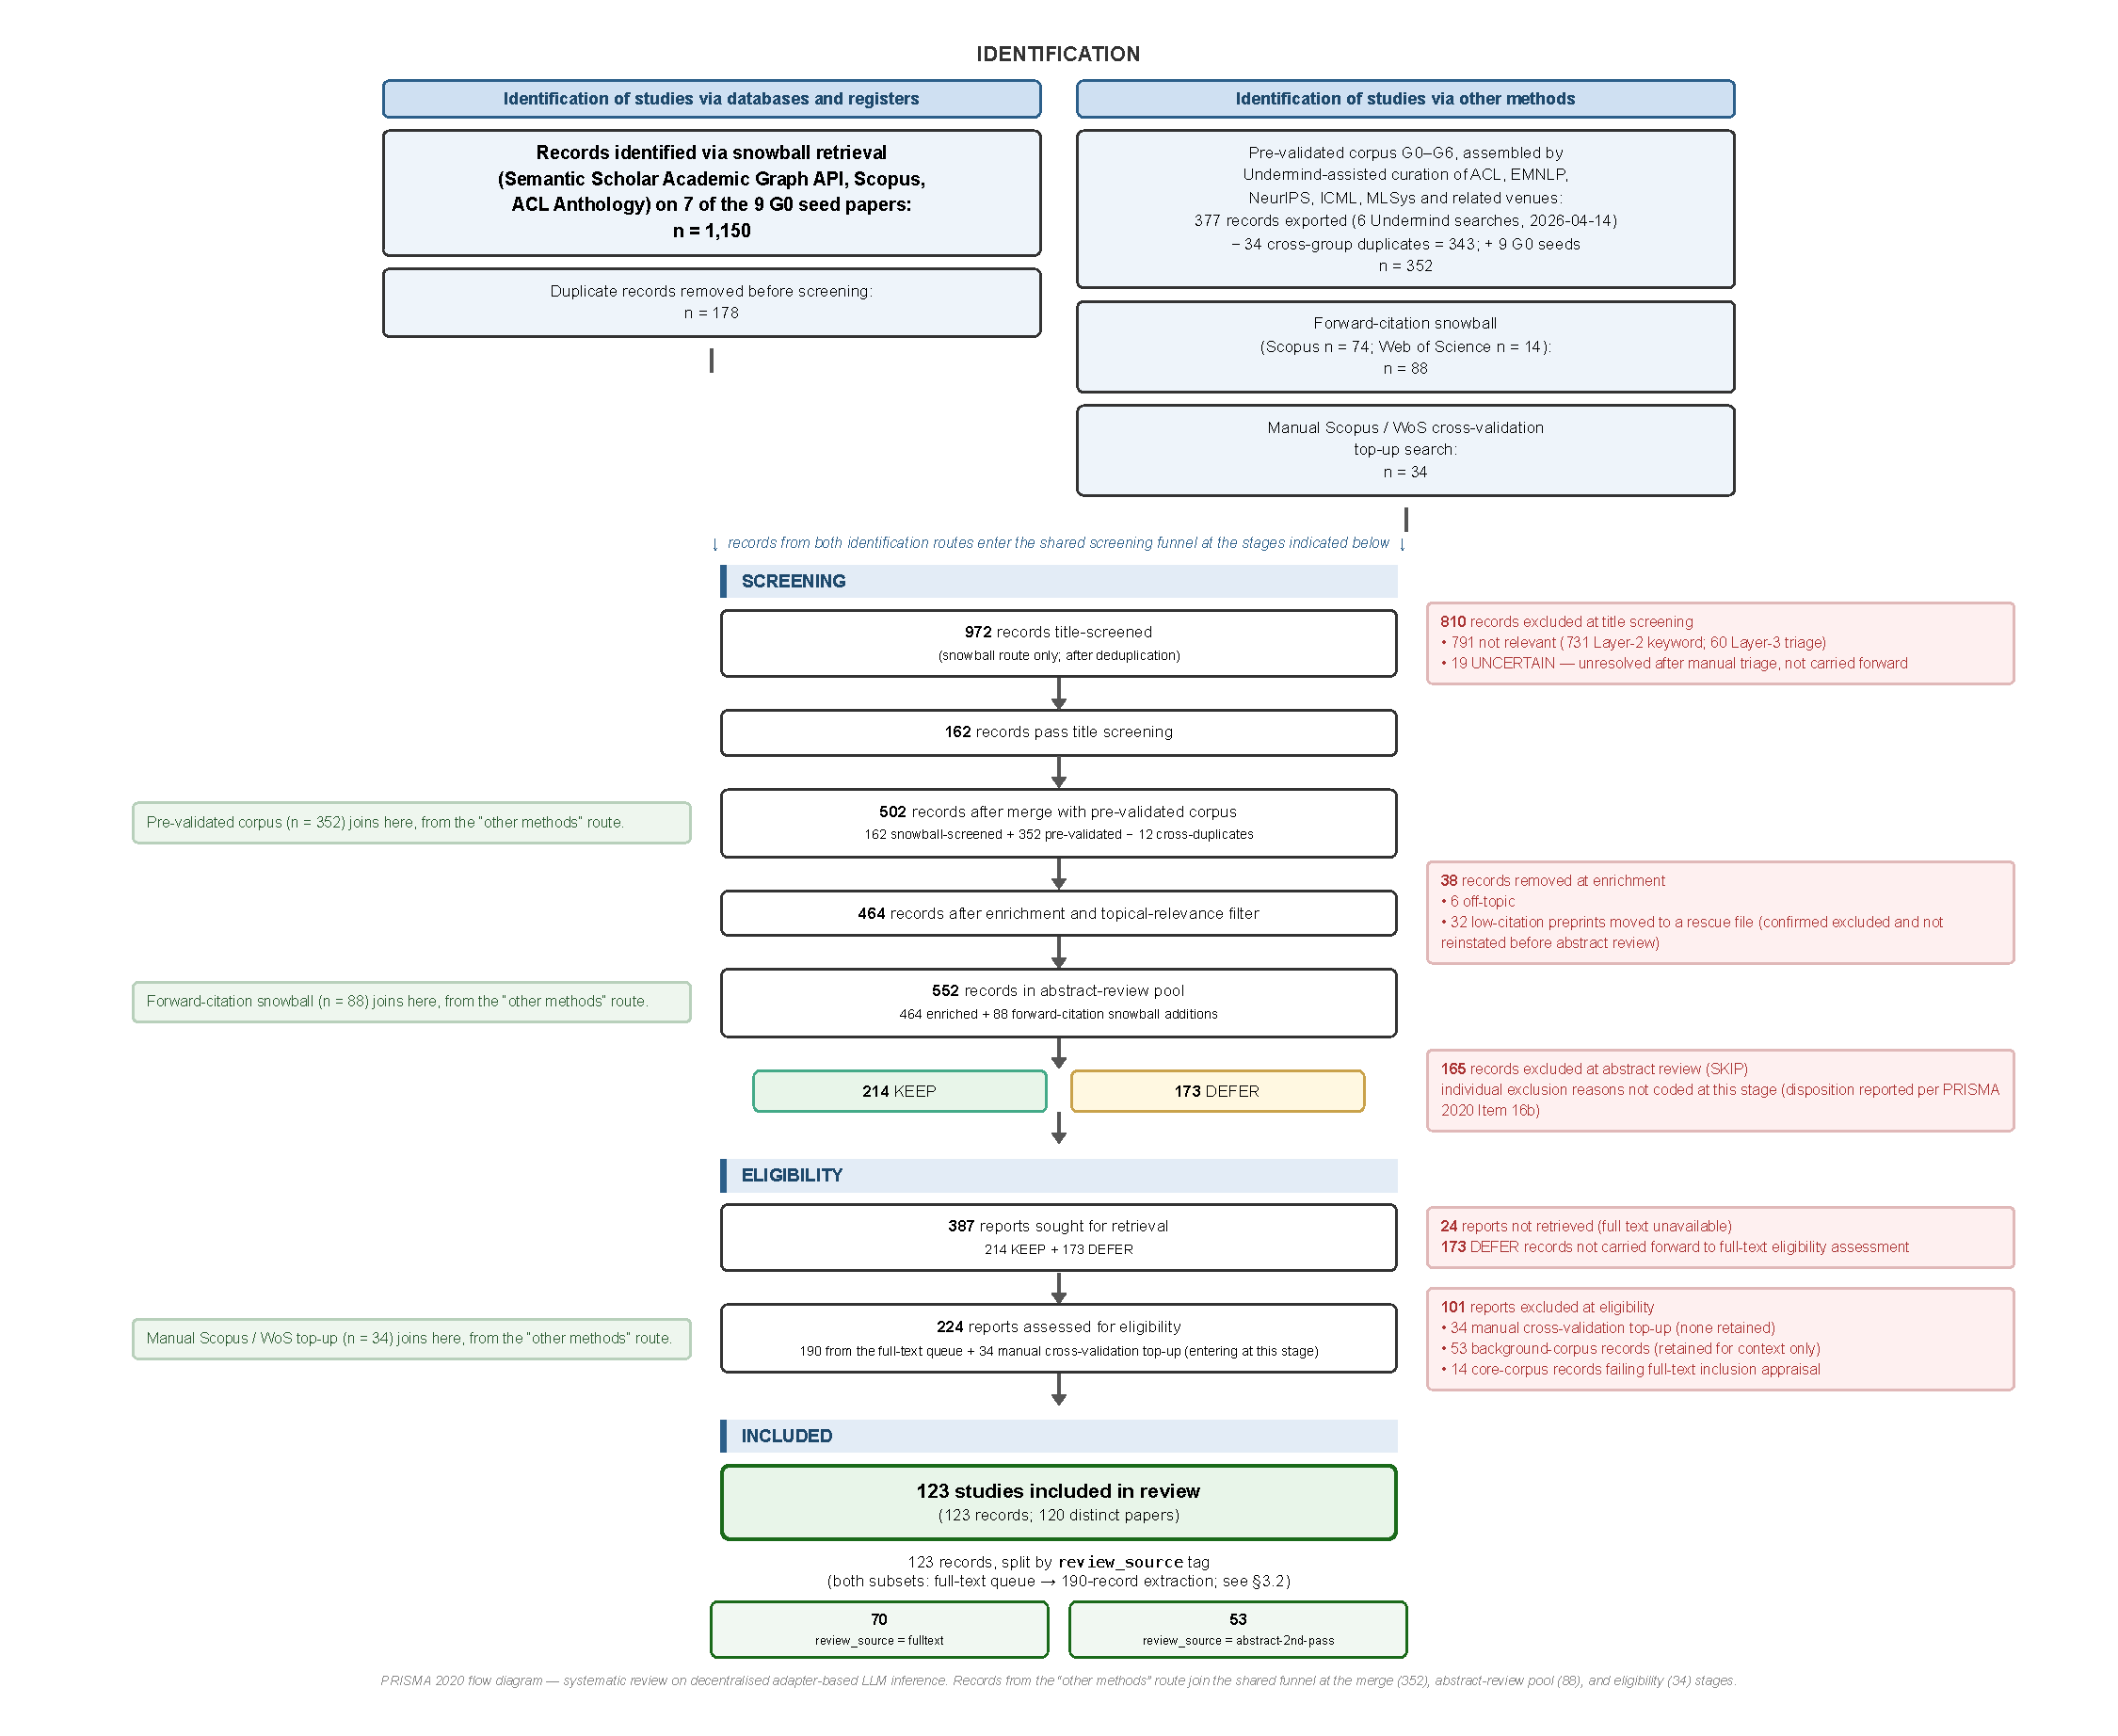
\includegraphics[width=\linewidth]{figures/fig_slr1_prisma_flow.pdf}
  \caption{PRISMA 2020 flow diagram (two-column variant). \emph{Left column ---
           identification via databases and registers:} one wave of
           forward/backward citation snowballing on seven of the nine G0 seeds
           (the two {\v{S}}ajina works were not submitted; see
           Table~\ref{tab:g0_disposition}), run
           through the Semantic Scholar Academic Graph API, Scopus, and ACL
           Anthology (\textbf{1,150} identified; \textbf{178} duplicates
           removed; \textbf{972} title-screened; \textbf{810} excluded ---
           \textbf{791} not relevant and \textbf{19} UNCERTAIN unresolved after
           triage; \textbf{162} retained). \emph{Right column ---
           identification via other methods:} the pre-validated G0--G6 corpus
           (\textbf{377} records exported from six Undermind deep searches
           ${}-{}$ \textbf{34} cross-group duplicates ${}={}$ \textbf{343};
           ${}+{}$ \textbf{9} G0 seeds ${}={}$ \textbf{352}, joining at the
           merge), a forward-citation snowball on
           Scopus and Web of Science (\textbf{88}, joining at the
           abstract-review pool), and a manual Scopus/WoS cross-validation
           top-up (\textbf{34}, joining at eligibility). The merged stream
           (\textbf{162} ${}+{}$ \textbf{352} ${}-{}$ \textbf{12}
           cross-duplicates ${}={}$ \textbf{502}) proceeds through enrichment
           and a topical-relevance filter (\textbf{502} ${}\rightarrow{}$
           \textbf{464}; \textbf{6} off-topic excluded and \textbf{32}
           low-citation preprints moved to a rescue file, confirmed excluded
           and not reinstated before abstract review), an abstract-review pool of
           \textbf{552} (\textbf{214} KEEP / \textbf{173} DEFER / \textbf{165}
           SKIP, the last excluded without individually coded reasons per
           PRISMA 2020 Item~16b), \textbf{387} reports sought for retrieval
           (\textbf{24} not retrieved; \textbf{173} DEFER not carried forward
           to full-text assessment), and \textbf{224} reports assessed for
           eligibility (\textbf{190} from the queue ${}+{}$ \textbf{34}
           top-up), of which \textbf{101} were excluded (\textbf{34} manual
           top-up, \textbf{53} background-corpus, \textbf{14} core-corpus
           failing full-text appraisal). The review includes \textbf{123}
           records (\textbf{120} distinct papers): \textbf{70} entered via
           full-text-queue assessment and \textbf{53} via a second
           abstract-review pass (\texttt{review\_source =
           abstract-2nd-pass}).}
  \label{fig:prisma}
\end{figure}

\subsection{Datasets and Benchmarks}
\label{sec:methodology:datasets}

Table~\ref{tab:datasets} reports the datasets, task types, and evaluation
metrics for 33 representative systems drawn from the five synthesis sections.
Its final \emph{Public} column records whether each system releases usable code
or artifacts (operational rule and check date in the caption).
PEFT papers predominantly evaluate on GLUE~\cite{WangGLUE2018},
SuperGLUE~\cite{WangSuperGLUE2019}, and MMLU~\cite{HendrycksMMLU2021};
serving papers rely on synthetic throughput benchmarks. No single benchmark
spans all three pillars simultaneously, a fragmentation that is itself one
of the empirical gaps identified in Section~\ref{sec:synthesis_gap}. The
representative ``Score'' figures are transcribed from the results reported in
the cited primary papers themselves (each row's cited reference is the source
of its reported value); they are not machine-mined from the extraction table,
whose quantitative benchmark columns are populated narratively rather than
from a parsed benchmark field. The figures are intended as indicative evidence
of evaluation practice and are not re-normalised or compared across papers.

\begin{sidewaystable}[p]
\centering
\caption{Selected datasets, tasks, and metrics across the five synthesis
pillars. The \emph{Public} column records \emph{code/artifact availability}:
whether the authors release usable source code or a functional artifact. Values
were re-derived for this revision by checking the cited systems' public
repositories on \textbf{2026-09-03}: \emph{Yes} = usable code/artifact located;
\emph{Partial} = available only through a maintained downstream framework rather
than the paper's own release (FedAvg, via TensorFlow Federated); \emph{No} = no
artifact released (Expert Choice, MT-EF); \emph{Unknown} = no public artifact
could be located at the check date (Ostapenko et al., DP-FedLoRA, SLoRA, Gossip
Learning). The column encodes artifact availability, not dataset availability:
the benchmarks themselves are public in every row.}
\label{tab:datasets}
\small
\setlength{\tabcolsep}{5pt}
  \resizebox{0.87\textwidth}{!}{%
  \begin{tabular}{lllllc}
  \toprule
  \textbf{Paper} & \textbf{Dataset} & \textbf{Task Type} & \textbf{Metric} &
  \textbf{Score} & \textbf{Public} \\
  \midrule
  \multicolumn{6}{l}{\textbf{Pillar 1: PEFT and Adapters}} \\
  Houlsby et al.~\cite{Houlsby2019} & GLUE, 17 add'l classification tasks & NLU
  classification & Accuracy & 80.0 (GLUE overall, BERT-large) & Yes \\
  Hu et al.~\cite{Hu2022} (LoRA) & GLUE & NLU classification & Accuracy &
  87.2 (GLUE avg., RoBERTa-base) & Yes \\
  Dettmers et al.~\cite{Dettmers2023} (QLoRA) & Vicuna benchmark & instruction
  following & Elo rating & 99.3\% of ChatGPT & Yes \\
  Li and Liang~\cite{LiLiang2021} (Prefix) & E2E, WebNLG, XSUM & NLG & ROUGE-L &
   36.05 (XSUM, BART-large, 2\% params) & Yes \\
  Ben-Zaken et al.~\cite{BenZaken2022} (BitFit) & GLUE & NLU classification &
  Accuracy & $\approx$ BERT-base full FT & Yes \\
  Poth et al.~\cite{PothAdapters2023} (Adapters lib.) & GLUE & NLU
  classification & Accuracy & matches full FT & Yes \\
  \midrule
  \multicolumn{6}{l}{\textbf{Pillar 2: Adapter Composition}} \\
  AdapterHub~\cite{Pfeiffer2020hub} & GLUE, XNLI & NLU + cross-lingual &
  Accuracy & multiple tasks & Yes \\
  AdapterFusion~\cite{Pfeiffer2021fusion} & 16-task suite (incl.\ MNLI, SciTail,
  MRPC, CB) & NLU classification & Accuracy & 94.8 (SciTail, Fusion w/ MT-A) & Yes \\
  MAD-X~\cite{PfeifferMADX2020} & NER, causal commonsense reasoning, QA
  (typologically diverse langs) & cross-lingual transfer &
  Accuracy/F1 & zero-shot transfer & Yes \\
  LoraHub~\cite{Huang2023} & BIG-Bench Hard & few-shot transfer & Accuracy &
  34.7 avg per task (BBH) & Yes \\
  LoraRetriever~\cite{ZhaoLoraRetriever2024} & domain QA, MT-bench & multi-task
   QA & Accuracy/win-rate & matches best single & Yes \\
  Ostapenko et al.~\cite{Ostapenko2024} & GLUE, SuperGLUE & NLU classification &
  Accuracy & --- & Unknown \\
  \midrule
  \multicolumn{6}{l}{\textbf{Pillar 3: Adapter-Aware Inference Serving}} \\
  S-LoRA~\cite{Sheng2024} & synthetic & throughput & req/s & up to 4$\times$
  throughput & Yes \\
  Punica~\cite{Chen2023Punica} & synthetic serving & throughput & req/s &
  12$\times$ higher throughput & Yes \\
  CaraServe~\cite{Li2024CaraServe} & synthetic & throughput & req/s &
  up to 1.7$\times$ & Yes \\
  Petals~\cite{Borzunov2023} & multiple & instruction following & Accuracy &
  multiple & Yes \\
  MT-EF (Multi-Task Encoder Fusion) / {\v{S}}ajina~\cite{Sajina2024} & Reddit, StackOverflow, CoNLL-2003,
  Few-NERD & MTP + NER & Test UA & +11.6\% mean relative gain & No \\
  \midrule
  \multicolumn{6}{l}{\textbf{Pillar 4: P2P and Federated Learning}} \\
  FedAvg~\cite{McMahan2017} & CIFAR-10, Shakespeare & image/text classification
   & Accuracy & 10--100$\times$ comm. saving & Partial \\
  FedProx~\cite{Li2020FedProx} & FEMNIST, Sent140 & image/text classification &
   Accuracy & +1--5\% vs FedAvg & Yes \\
  FedPETuning~\cite{ZhangFedPETuning2023} & GLUE & NLU classification &
  Accuracy & $\leq$5\% loss vs central PEFT & Yes \\
  FLoRA~\cite{WangFLoRA2024} & GLUE (few-shot) & NLU classification & Accuracy
  & robust to rank hete. & Yes \\
  DP-FedLoRA~\cite{XuDPFedLoRA2025} & MMLU, BBH, CRASS & NLU + reasoning &
  Accuracy + $(\epsilon,\delta)$ & $\approx$4--5\% loss at $\epsilon=25$ & Unknown \\
  SLoRA~\cite{Babakniya2023} & GLUE, SuperGLUE & NLU classification & Accuracy
  & 2$\times$ faster convergence & Unknown \\
  Gossip Learning~\cite{HegeduisGossip2019} & synthetic & classification &
  Accuracy & $\approx$ FL quality (compression-rate-dependent: slower
  uncompressed, competitive-to-faster under high compression) & Unknown \\
  \midrule
  \multicolumn{6}{l}{\textbf{Pillar 5: MoE and Adapter Routing}} \\
  Switch Transformers~\cite{Fedus2022} & C4 pre-training & language modelling &
   Perplexity, speedup & 4$\times$ speedup over T5-XXL & Yes \\
  Expert Choice~\cite{Zhou2022} & SuperGLUE, WMT & NLU + MT & Accuracy/BLEU &
  +2\% average accuracy & No \\
  DeepSpeed-MoE~\cite{RajbhandariDeepSpeed2022} & GLUE, SuperGLUE & NLU
  classification & Accuracy & 4.5$\times$ speedup, $<$0.5\% loss & Yes \\
  AdaMix~\cite{WangAdaMix2022} & GLUE, SuperGLUE & NLU classification &
  Accuracy & outperforms single PEFT & Yes \\
  MixLoRA~\cite{LiMixLoRA2024} & GLUE, domain-specific & NLU classification &
  Accuracy & --- & Yes \\
  MiLoRA~\cite{ZhangMiLoRA2024} & commonsense reasoning, math reasoning &
  reasoning + instruction following & Accuracy & $>$ single LoRA & Yes \\
  LoRAMoE~\cite{DouLoRAMoE2024} & world knowledge + instruct & multi-task
  generation & Accuracy, forgetting & alleviates forgetting & Yes \\
  MOELoRA (Liu et al.)~\cite{LiuWhenMOE2024} & medical + GLUE & NLU classification &
  Accuracy & $>$ single LoRA & Yes \\
  Crowdsourced MoE~\cite{RyabininCrowdsourced2020} & CIFAR-10/100, MNIST &
  image classification & Accuracy & up to 16 peers, 30\% dropout & Yes \\
\bottomrule
  \end{tabular}
  }
\end{sidewaystable}

\subsection{Reporting-Completeness and Relevance Appraisal}
\label{sec:methodology:quality}

Because the review is a qualitative thematic synthesis of published
methods--and--systems literature rather than a meta-analysis of participant-level
interventions, the PRISMA 2020 risk-of-bias instruments for comparative studies do
not apply directly.

This review therefore does not claim to have conducted a classical risk-of-bias
assessment as defined for comparative clinical or empirical intervention studies.
Its object of appraisal is the reporting quality and synthesis relevance of
methods-and-systems papers, not the internal validity of a controlled comparison.
Where the reviewed literature permits it, this review supplements the
reporting-completeness rubric with a targeted, verified reproducibility check
(code/artifact availability, Section~\ref{sec:methodology:quality:tier1}) over a
representative subset of 33 systems; this subset check is disclosed as a bounded,
illustrative appraisal and not extrapolated as a corpus-wide risk-of-bias
statistic.

Following the practice of software-literature systematic
reviews~\cite{XiaoWatson2019}, this review instead appraises the \emph{reporting
completeness and thematic relevance of each of the 123 included records} with a
six-dimension rubric scored
from the screening and extraction records (Table~\ref{tab:quality_rubric}). It is
emphasised that this instrument measures the reporting completeness of each record
and its relevance to this synthesis, not the intrinsic scientific merit of the
underlying study: three dimensions are bibliographic or relevance proxies (Q1
venue prestige, Q2 record resolvability, Q6 thematic relevance), and a pilot
application of the classic quality dimensions (code availability, result
reproducibility, baseline adequacy, threats reporting) found them to be
un-populated in the extraction data, so they are scoped out here and disclosed
rather than estimated. The \texttt{contribution\_codes} field underlying the top
tier of Q5 is itself sparsely populated (22 of 224 extraction rows, 9.8\%). Records
lacking a populated \texttt{contribution\_codes} field are excluded from the Q5
sub-score rather than defaulted to the middle tier; Q5 is therefore reported only
over the subpopulation of the 123 retained records where the field is populated
($n=16$; the 22 populated extraction rows reduce to 16 distinct retained records
after deduplication onto the final list), and this should be read as a limitation
of extraction coverage rather than a substantive quality signal. Every retained
dimension is nevertheless operationalised from an explicit, grounded pipeline field
so that each score is reproducible from the associated CSV artifacts; no dimension
is inferred or imputed.

\begin{table}[htp]
\centering
\caption{Reporting-completeness and relevance rubric: each dimension is scored 0--2 from a grounded
screening/extraction field. The reporting-completeness total is the sum of Q1--Q4 and Q6 (0--10);
Q5 is scored separately and is excluded from the total.}
\label{tab:quality_rubric}
\small
\setlength{\tabcolsep}{3pt}
\begin{tabular}{
  >{\raggedright\arraybackslash}p{0.17\textwidth}
  >{\raggedright\arraybackslash}p{0.29\textwidth}
  >{\centering\arraybackslash}p{0.14\textwidth}
  >{\centering\arraybackslash}p{0.14\textwidth}
  >{\centering\arraybackslash}p{0.14\textwidth}}
\toprule
\textbf{Dimension} & \textbf{Grounded source} & \textbf{0} & \textbf{1} & \textbf{2} \\
\midrule
Q1 Publication \& venue quality & Venue-quality tag (preprint /
peer-reviewed / top venue) & preprint & peer-reviewed & top venue \\
Q2 Record resolvability & Presence of a DOI and/or arXiv ID (union of the
final list, enriched pool, and extraction table) & neither & one & both \\
Q3 Methods specificity & Named PEFT technique in extraction +
identifiable method in full-text notes & generic/absent technique & named
technique & named method with specific PEFT technique \\
Q4 Evaluation-claim specificity & Key finding / full-text notes & no claim &
structural or qualitative claim & quantified or benchmarking claim \\
Q5 Contribution clarity & Contribution type + contribution code(s) &
neither & contribution type only & contribution type + \ccstar~code(s) \\
\addlinespace
\multicolumn{5}{l}{\footnotesize\emph{Q5 is scored only where \texttt{contribution\_codes} is populated and is reported separately; it is not included in the 0--10 total.}} \\
Q6 Synthesis relevance & Tier (1 = core PEFT+P2P+LLM, \dots, 3 =
tangential) & tier 3 & tier 2 & tier 1 \\
\bottomrule
\end{tabular}
\end{table}

Applying the rubric to the 120 distinct studies underlying the 123 final
records\footnote{Three works are each scored twice under two record
identities (arXiv preprint and peer-reviewed/Scopus release): LoRA, Houlsby's
adapter paper, and CaraServe/Toppings. These duplicate pairs are not scored
identically (verified in \texttt{verify/wp9\_appraisal\_n\_and\_totals.py}:
LoRA 8/8, Houlsby 5/6, CaraServe/Toppings 7/6), so the appraisal reported here
retains one row per study --- its arXiv-keyed record for LoRA and Houlsby, its
peer-reviewed record for CaraServe/Toppings --- rather than scoring the same
study twice.} yields a mean reporting-completeness
score of $6.03$ ($\mathrm{SD}=2.01$, median 6), with the distribution
summarised in Figure~\ref{fig:quality_bands}: 13 records (10.8\%) fall in the
high band (9--10), 59 (49.2\%) in the upper-mid band (6--8), 46 (38.3\%) in the
lower-mid band (3--5), and 2 (1.7\%) in the low band (0--2). Q5 is excluded
from these totals and reported separately over its populated subpopulation
($n=16$), all of which recorded a contribution type and \ccstar~code(s).
The full record-by-record scores for all 123 records (including both rows of
each duplicate pair) are provided as accompanying material in
\texttt{figures/quality\_appraisal\_scored.csv}; the 120-distinct-study subset
used for the statistics above is
\texttt{verify/wp9\_quality\_appraisal\_120\_studies.csv} (each scored
0--2 on Q1--Q4 and Q6 with a reporting-completeness total of 0--10, and Q5
reported separately). The low-scoring records are
pre-PEFT-era distributed-optimisation works (e.g.\ decentralised and gossip
cooperative learning) that are tangential to the modern adapter-based core; none
of the findings reported in Sections~\ref{sec:peft} to~\ref{sec:synthesis_gap}
rests on a low-scoring record alone.

\begin{figure}[htbp]
\centering
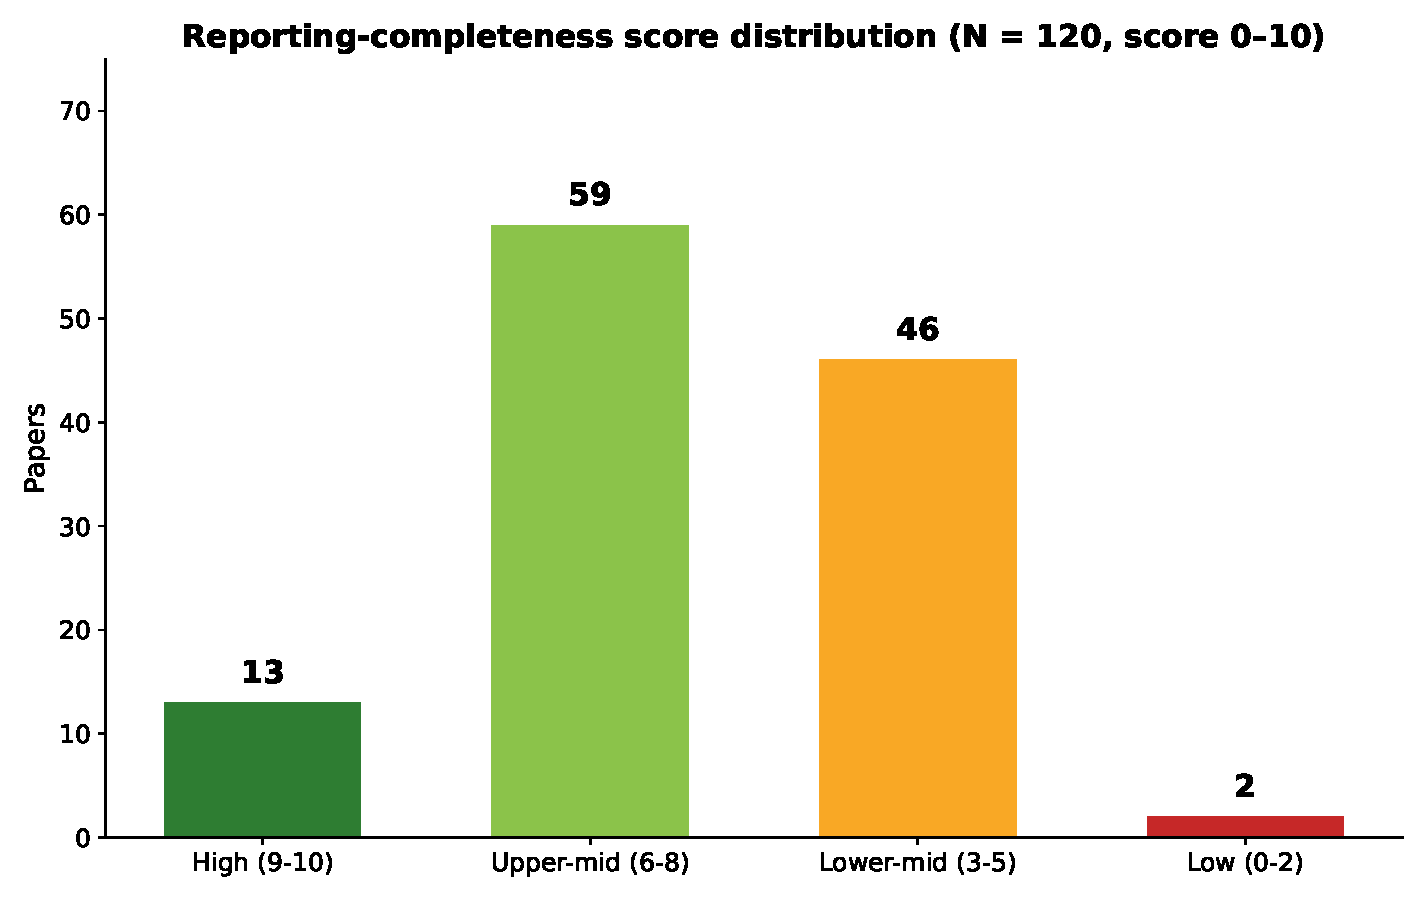
\includegraphics[width=0.92\linewidth]{figures/fig_slr_quality_bands.pdf}
\caption{Reporting-completeness score distribution across the 120 distinct
studies underlying the 123 included records
(0--10 rubric: Q1--Q4 and Q6 summed; Q5 reported separately).}
\label{fig:quality_bands}
\end{figure}

\subsubsection{Reproducibility: Artifact Availability}
\label{sec:methodology:quality:tier1}

Whereas the six-dimension rubric above scores reporting completeness and
relevance across all 123 records, three further dimensions central to
empirical reproducibility: \emph{code/artifact availability}, \emph{baseline
adequacy}, and \emph{explicit threats-to-validity reporting}, require
full-text inspection that lies beyond the automated screening pipeline. Of
these, this review reports \emph{code/artifact availability} quantitatively,
grounded in verified evidence: for each of the 33 representative systems in
Table~\ref{tab:datasets}, the author checked directly against the system's
public repositories whether usable code or an artifact is released (the
operational rule and check date are stated in the table caption). Baseline
adequacy and threats-to-validity reporting are likewise central to risk of
bias, but the review's screening and extraction records do not populate
reliable per-record codings for these two dimensions, so no quantitative claim
is made for them here; reporting figures would have imputed rather than
measured. They remain a candidate for a full-text re-read pass before
submission.

The verified picture is uneven. Across the 33 representative systems,
\textbf{26} (\textbf{79\%}) release usable code or artifacts, and \textbf{1}
(\textbf{3\%}), FedAvg, is available only through a maintained downstream
framework (TensorFlow Federated) rather than its original release. For
\textbf{2} systems (\textbf{6\%})---Expert Choice and MT-EF
({\v{S}}ajina et al.)---no artifact was located at the check date; for a further
\textbf{4} systems (\textbf{12\%})---Ostapenko et al., DP-FedLoRA, SLoRA, and
Gossip Learning---no public artifact could be located at the check date
either, which does not rule out an unreleased or unadvertised one existing. The gap is concentrated among the systems closest to this
review's object of study: three of the seven federated or P2P fine-tuning
methods in Pillar 4 (SLoRA, DP-FedLoRA, Gossip Learning), the MT-EF P2P architecture, and
the modular-LoRA composition framework (Ostapenko et al.) have no locatable
artifact at the check date, despite several being recent and otherwise well-documented.

These findings are themselves a result of this review. The unevenness (in
particular the absence of locatable artifacts for several systems most central
to the P2P and adapter-composition directions) substantiates, at the level of
primary evidence, the reproducibility and reporting gaps identified in
Section~\ref{sec:synthesis_gap}, and it informs the gap analysis in
Section~\ref{sec:conclusion:contributions}. These dimensions remain outside the
0--10 reporting-completeness rubric by design and are reported here as a
separate, clearly-labelled appraisal rather than folded into the aggregate
score. The per-row artifact-availability codings are given in
Table~\ref{tab:datasets}.
